\subsection{Relay Cluster Deployment}

A Databus deployment consists of a cluster of relay servers that pull the change stream from multiple database servers. Each relay server can connect to multiple database servers and host the change stream from each server in separate buffers in the same relay. The relays are also set up in such a way that the change stream from every database server is available in multiple relays, for fault-tolerance and for consumer scaling. There are two configurations the relays are typically deployed.

\begin{figure}
\centering
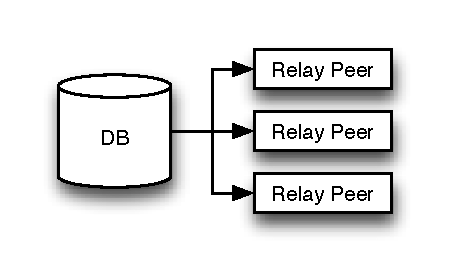
\epsfig{file=figures/relay_deployment_peers.eps, width=2.5in}
\caption{Independent Relays Deployment}
\label{fig:RelayDeployment1}
\end{figure}

In one deployment model as shown in Figure \ref{fig:RelayDeployment1}, all the relay servers connect to the source database server. Each relay server is assigned a subset of the database streams. The relay connects to the specified database servers and pulls the change streams. When a relay fails, the surviving relays continue pulling the change streams independent of the failed relay. If the configured redundancy factor is R, this model provides 100\% availability of the streams at very low latency as long as all the R relays that connect to the same database server do not fail at the same time. This however comes as the cost of increased load on the database server since there are R relays that pull the same change stream.

\begin{figure}
\centering
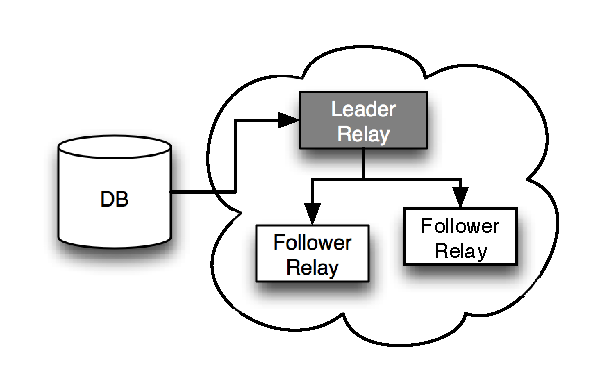
\epsfig{file=figures/relay_deployment_leader.eps, width=3in}
\caption{Leader-Followers Relays Deployment}
\label{fig:RelayDeployment2}
\end{figure}

To reduce the load on the source database server, an alternative deployment model for relays as shown in Figure \ref{fig:RelayDeployment2}, is the Leader-Follower model. In this model, for every database server, one relay is designated to be the leader while R-1 are designated to be followers. The leader relay connects to the database to pull the change stream while the follower relays pull the change stream from the leader. The clients can connect to any of the relays, either leader or follower. If the leader relay fails, one of the surviving followers is elected to be the new leader. The new leader connects to the database server and continues pulling the change stream from the last sequence number it has. The followers disconnect from the failed leader and connect to the new leader. This deployment drastically reduces the load on the database server but when the leader fails, there is a small delay while a new leader is elected. During this window, the change stream from the database server is not available to the consumers.

To expand capacity of, new relay servers can be added to the cluster. When this happens, a new assignment of database servers to relay servers is generated so that some streams are transferred from the old relay servers to the new relay servers. The new relay servers then connect to the database servers and start pulling the change streams. They can optionally copy the existing change streams from the old relay servers before connecting to the database servers. Management of the relay cluster is done using a generic cluster manager built at LinkedIn called Helix.

The assignment of databases to relays is made available to databus consumers in the form of a routing table so that the clients can discover the location of the streams they wish to consume. When the assignment changes due to relay failures or relay cluster rebalancing, this routing table is automatically updated and the consumers switch to the new servers transparently.

\subsection{Partitioned Stream Consumption}

Databases are often partitioned horizontally for scalability. As the read and write load changes, databases will get repartitioned repeatedly. A consumer who is subscribing to the change stream from a database must be able to do so independent of the partitioning of the database. Often the change stream will be too fast for a single consumer to process and the processing needs to be scaled out across multiple physical consumers who act as a logical group. In case of partitioned sources,  currently Databus enforces the transactional semantics only at the partition level. 

Databus implements the notion of a consumer group, using the generic cluster manager Helix. The partitions of the database are assigned to the consumers in the same group so that every partition has one and exactly one consumer in the group assigned to it and the partitions are evenly distributed among the consumers. When any consumer fails, Helix rebalances the assignment of partitions by moving the partitions assigned to the failed consumer to the surviving consumers. If the existing consumers in the group are not able to keep up with the stream, additional consumers might be added to the group to scale the processing. In this case, the assignment of partitions is rebalanced so that some partitions from each existing consumer are moved to the new consumers.

